\subsection{Post-starburst (PSB) Galaxies}
\label{sec:PSBs}
Vivienne has been involved in the preparation of a number of papers researching PSBs: \citet{2017MNRAS.472.1401A} regarding the relationship between quenching of star formation and morphological transition, while \citet{2016MNRAS.463..832W} sets out the background work.
\par Galaxy evolution has been explained by many authors [TODO: expand to create a list] \citep{baldry2004quantifying,2006MNRAS.373..469B} by referring to a galaxy colour-magnitude diagram (CMD) as illustrated in Fig.~\ref{fig:CMD1}. Young blue, often spiral, galaxies in the lower-right 'blue cloud' region are understood to transition to the redder mainly early-type elliptical quiescent galaxies along the upper left 'red sequence' region of the CMD. There is a sparsely populated region separating the two populations: this is often referred to as the 'green valley' region \citep{2004ApJ...608..752B}. In this paper we explore galaxies in transition between the blue cloud and the red sequence, through the green valley.
\citet{Mutch_2011} assert that both the Milky Way and the Andromeda galaxy M31 are in transition and lie within the green valley region of the galaxy CMD.

\begin{figure}
	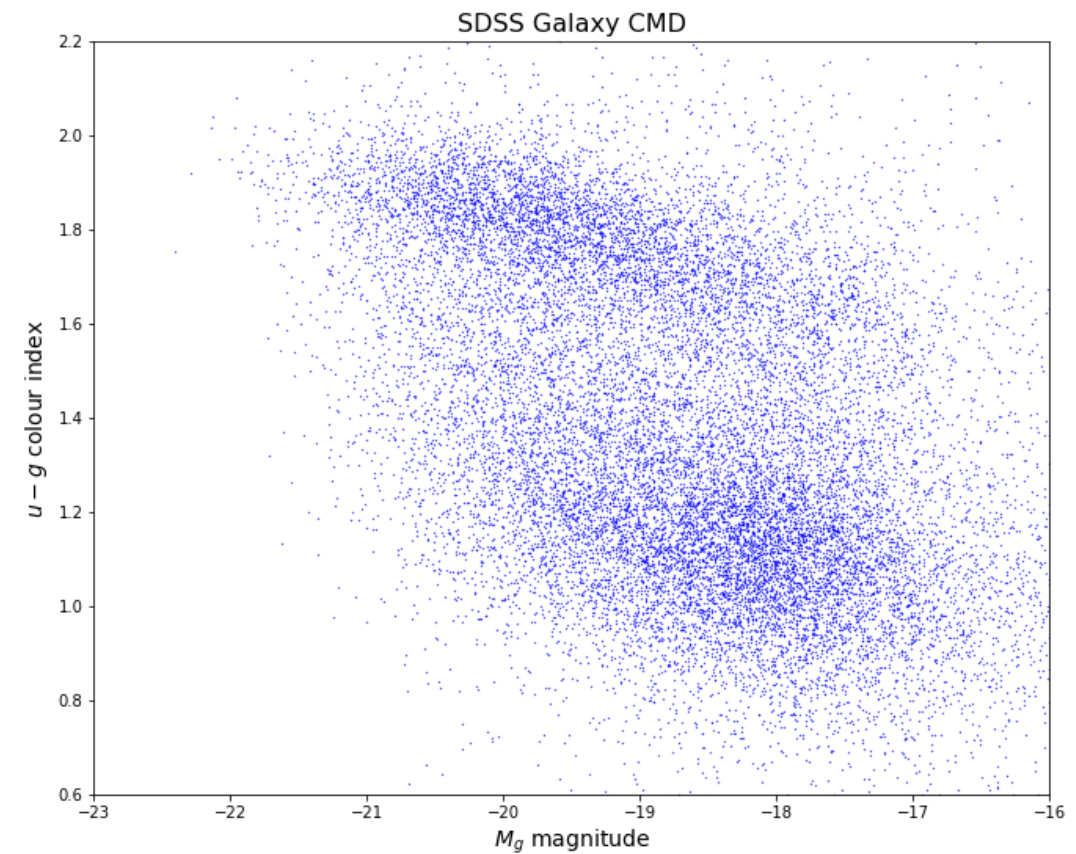
\includegraphics[width=\columnwidth]{images/CMDs/galaxyCMD.PNG}
    \caption{Galaxy colour-magnitude diagram: $u-g$ colour index versus $M_g$ magnitude. The bimodality of the distribution is discussed in the text.}
    \label{fig:CMD1}
\end{figure}